% Intended LaTeX compiler: pdflatex
\documentclass[t]{beamer}
\usepackage[utf8]{inputenc}
\usepackage[T1]{fontenc}
\usepackage{graphicx}
\usepackage{grffile}
\usepackage{longtable}
\usepackage{wrapfig}
\usepackage{rotating}
\usepackage[normalem]{ulem}
\usepackage{amsmath}
\usepackage{textcomp}
\usepackage{amssymb}
\usepackage{capt-of}
\usepackage{hyperref}
\usepackage{listings}
\usepackage{xcolor}
\usepackage[french, frenchb]{babel}
% typeset source code listings
\usepackage{listings}
\usepackage{xcolor}
\definecolor{mc@lstidentifier}{HTML}{000000} % black
\definecolor{mc@lstcomment}{HTML}{008200} % green
\definecolor{mc@lststring}{HTML}{FF5500} % orange
\definecolor{mc@lstkeyword}{HTML}{0000FF} % blue
\definecolor{mc@lstbackground}{HTML}{FFFFCC} % light yellow
\definecolor{mc@lstframe}{HTML}{FFEE88} % dark yellow
\lstdefinelanguage{org}{%
morekeywords={:results, :session, :var, :noweb, :exports},
sensitive=false,
morestring=[b]",
morecomment=[l]{\#},
}
\lstset{%
lineskip=-0.1em,
%
basicstyle=\ttfamily\scriptsize, % font that is used for the code
identifierstyle=\color{mc@lstidentifier},
commentstyle=\color{mc@lstcomment}\itshape,
stringstyle=\color{mc@lststring},
keywordstyle=\color{mc@lstkeyword},
%
extendedchars=true,
inputencoding=utf8,
upquote, %
tabsize=4, % set default tabsize to 4 spaces
showtabs=false, % show tabs within strings adding particular underscores
%  tab=$\to$,
showspaces=false, % show spaces adding particular underscores
showstringspaces=false, % underline spaces within strings
%
numbers=left, % where to put the line numbers
stepnumber=0, % step between two line numbers
numberstyle=\tiny, % line number font size
%
captionpos=b, % set the caption position to `bottom'
%
xleftmargin=0.4em, % text to the right
xrightmargin=0.4em, % text to the left
breaklines=false, % don't break long lines of code
%
frame=single, % add a frame around the code
framexleftmargin=0pt, % frame back to the left
framexrightmargin=0pt, % frame back to the right
backgroundcolor=\color{mc@lstbackground}, % set the background color
rulecolor=\color{mc@lstframe}, % frame color
%
columns=flexible, % try not to ruin the spacing intended by the font designer
keepspaces=true, % don't drop spaces to fix column alignment
%
% mathescape, % allow escaping to (La)TeX mode within $..$
escapechar=², % allow escaping to (La)TeX mode within ²..²
% The backquote was NOT judicious: in some code (comments), I wrap vars
% between such a backquote (`var')
%
% conversion of UTF-8 chars to latin1
literate=
{á}{{\'a}}1
{à}{{\`a}}1
{â}{{\^a}}1
{ä}{{\"a}}1
{ç}{{\c{c}}}1
{é}{{\color{black}\'e}}1
{è}{{\`e}}1
{ê}{{\^e}}1
{ë}{{\"e}}1
{í}{{\'i}}1
{ì}{{\`i}}1
{î}{{\^i}}1
{ï}{{\"i}}1
{ó}{{\'o}}1
{ò}{{\`o}}1
{ô}{{\^o}}1
{ö}{{\"o}}1
{ú}{{\'u}}1
{ù}{{\`u}}1
{û}{{\^u}}1
{ü}{{\"u}}1
{Á}{{\'A}}1
{À}{{\`A}}1
{Â}{{\^A}}1
{Ä}{{\"A}}1
{Ç}{{\c{C}}}1
{É}{{\'E}}1
{È}{{\`E}}1
{Ê}{{\^E}}1
{Ë}{{\"E}}1
{Í}{{\'I}}1
{Ì}{{\`I}}1
{Î}{{\^I}}1
{Ï}{{\"I}}1
{Ó}{{\'O}}1
{Ò}{{\`O}}1
{Ô}{{\^O}}1
{Ö}{{\"O}}1
{Ú}{{\'U}}1
{Ù}{{\`U}}1
{Û}{{\^U}}1
{Ü}{{\"U}}1
}
\definecolor{TeXbackgroundcolor}{HTML}{F1F9EF}
\definecolor{TeXrulecolor}{HTML}{D4E8E3}
\lstdefinestyle{TeX}{backgroundcolor=\color{TeXbackgroundcolor},rulecolor=\color{TeXrulecolor}}
\definecolor{mylinkcolor}{HTML}{006DAF}
\hypersetup{colorlinks=true, linkcolor=mylinkcolor, urlcolor=mylinkcolor}
\usepackage{nccparskip}
\SetParskip{6pt plus 1pt minus .4pt}
\usepackage{menukeys}
\let\ORIkeys\keys
\renewcommand{\keys}[1]{\ORIkeys{\texttt{#1}}}
\newcommand{\repeatedkeys}[1]{\keys{\textcolor{gray}{#1}}}
\usetheme{default}
\author{\href{mailto:fniessen@pirilampo.org}{Fabrice Niessen}}
\date{28 juin 2017}
\title{Emacs + AUCTeX}
\subtitle{Le meilleur éditeur pour \LaTeX}
\institute[Pirilampo]{}
\titlegraphic{
\includegraphics[height=1.5cm]{images/Pirilampo}}
\AtBeginSection{%
\begin{frame}
\frametitle{Plan}
\tableofcontents[currentsection]
\end{frame}
}
\AtBeginSubsection{%
\begin{frame}
\frametitle{Plan}
\tableofcontents[currentsection,currentsubsection]
\end{frame}
}
\usepackage{lmodern}
\usetheme{AnnArbor}
\usecolortheme{crane}
\beamertemplatenavigationsymbolsempty
\hypersetup{
 pdfauthor={\href{mailto:fniessen@pirilampo.org}{Fabrice Niessen}},
 pdftitle={Emacs + AUCTeX},
 pdfkeywords={},
 pdfsubject={},
 pdfcreator={Emacs 25.2.1 (Org mode 9.0.8)}, 
 pdflang={Frenchb}}
\begin{document}

\title{Emacs + AUC\TeX{}}
\date[juin 2017]{28 juin 2017}
\begin{frame}[plain]
\maketitle
\end{frame}
\begin{frame}{Plan}
\tableofcontents
\end{frame}


\section{Aperçu}
\label{sec:org1898530}

\begin{frame}[label={sec:orgfee56ab}]{Description}
Bienvenue dans le cours Emacs + AUC\TeX{}. Il contient la documentation de
référence qui décrit comment écrire du code \LaTeX{} avec :

\begin{itemize}
\item l'éditeur GNU Emacs et
\item la librairie AUC\TeX{}.
\end{itemize}

Ces outils \alert{libres} et \alert{gratuits} vous permettent de produire facilement des
documents \alert{PDF de haute qualité} qui vont être affichés sur tous les ordinateurs
exactement comme ils l'étaient sur le vôtre.
\end{frame}

\begin{frame}[label={sec:orgf5f95e6}]{Caractéristiques et objectifs}
Les avantages évidents d'utiliser Emacs + AUC\TeX{} sont d'être \alert{plus productif}
pour éditer du \LaTeX{}.

À côté de fonctions standards comme la navigation aisée dans le document ou la
vérification orthographique et syntaxique à la volée, Emacs offre des
\alert{fonctionnalités avancées} (et homogènes) pour tout \alert{type de fichiers}. Par
exemple :

\begin{itemize}
\item recherche incrémentale,
\item édition de rectangles,
\item macros,
\item Helm.
\end{itemize}
\end{frame}

\begin{frame}[label={sec:org431cdac}]{Exigences}
\begin{itemize}
\item Une version d'Emacs 25 (si possible).

\item Une installation fonctionnelle de \LaTeX{} est requise pour exporter vers du
PDF. Si elle n'est pas encore installée sur votre système, installer \href{http://www.tug.org/texlive/}{\TeX{} Live}
(par exemple).
\end{itemize}
\end{frame}

\begin{frame}[label={sec:orgdde5f78}]{Besoin de plusieurs outils dans votre boîte}
\begin{figure}[!htbp]
\centering
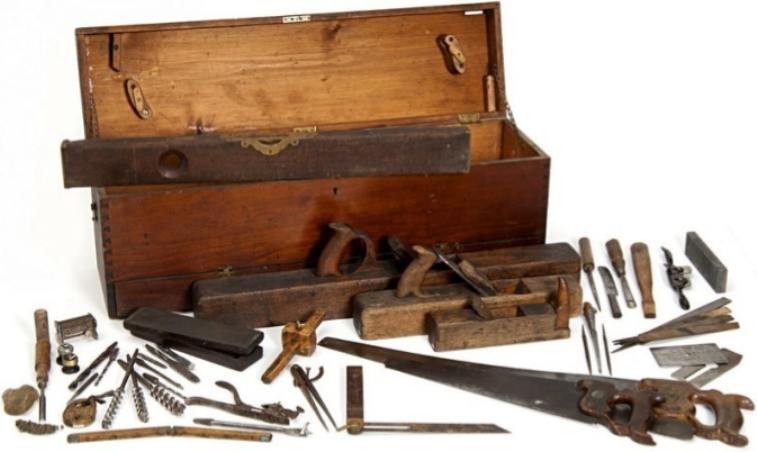
\includegraphics[width=.75\linewidth]{images/toolbox-messy.png}
\end{figure}
\end{frame}

\begin{frame}[label={sec:orgc16c756}]{Emacs intègre tous ces outils}
\begin{columns}
\begin{column}{0.57\columnwidth}
\begin{itemize}
\item Très puissant
\item Générique et spécialisé (environnement de développement pour beaucoup de
langages, gestionnaire de fichiers, terminal \emph{shell}, client mail, navigateur
Web, client IRC, Tetris, etc.)
\item Complètement extensible et personnalisable (en Lisp)
\end{itemize}
\end{column}

\begin{column}{0.4\columnwidth}
\begin{center}
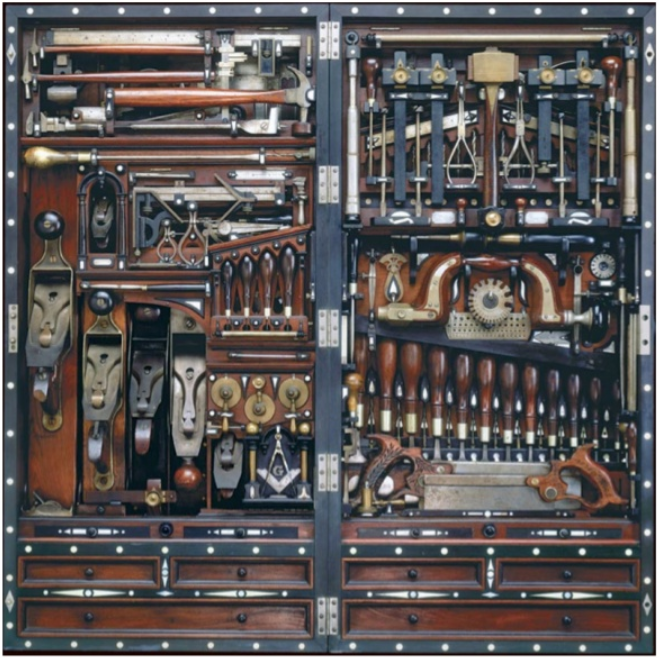
\includegraphics[width=\linewidth]{images/toolbox-tidy.png}
\end{center}
\end{column}
\end{columns}

\begin{itemize}
\item Libre et gratuit
\item Multi-plate-forme (Linux, MacOS, Windows)
\end{itemize}
\end{frame}

\begin{frame}[label={sec:orga263d8a}]{Productivité = capacité à ÉDITER DU TEXTE}
Emacs ne devrait pas être vu comme un éditeur : c'est un environnement de
développement logiciel avec de \alert{puissantes capacités d'édition de texte}. Et
c'est même encore beaucoup plus que cela !

\begin{quote}
« Emacs outshines all other editing software in approximately the same way that
the noonday sun does the stars. It is not just bigger and brighter; it simply
makes everything else vanish. » \\
--- Neal Stephenson, \\
\emph{In the Beginning was the Command Line} (1998)
\end{quote}

Emacs est mon outil \alert{le plus important} !
\end{frame}

\section{Bases pour utiliser Emacs}
\label{sec:org3d77968}

\begin{frame}[label={sec:orgb431086}]{Terminologie Emacs}
\begin{figure}[!htbp]
\centering
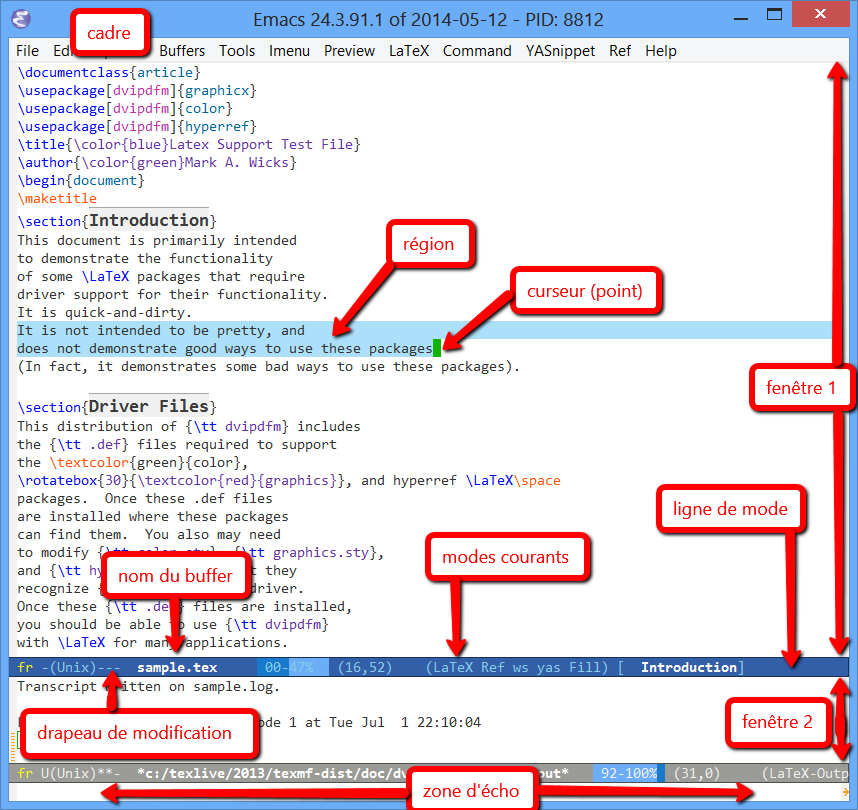
\includegraphics[width=.65\linewidth]{images/emacs-labeled.png}
\end{figure}
\end{frame}

\begin{frame}[label={sec:org4be1382}]{Ne pas utiliser la souris}
\begin{figure}[!htbp]
\centering

\includegraphics[width=.9\linewidth]{images/elephants.png}
\end{figure}
\end{frame}

\begin{frame}[label={sec:org82050cb}]{Exemple de fichier \LaTeX{} sous Emacs}
\begin{figure}[!htbp]
\centering
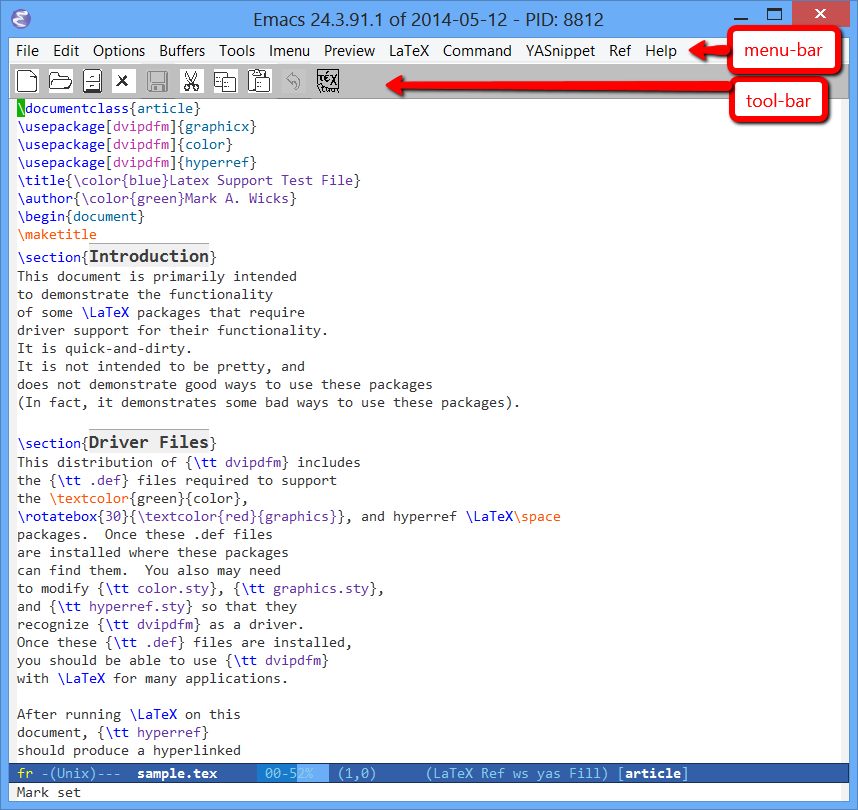
\includegraphics[width=.65\linewidth]{images/toolbar.png}
\end{figure}
\end{frame}

\begin{frame}[label={sec:org900a573}]{Notation des raccourcis clavier}
\begin{figure}[!htbp]
\centering
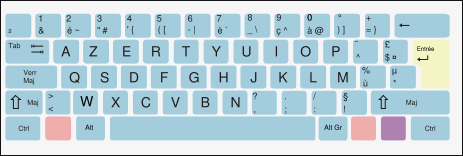
\includegraphics[width=.5\linewidth]{images/clavier_azerty.png}
\end{figure}

\begin{itemize}
\item Touches spéciales (modificateurs) :
\begin{description}
\item[{\keys{S}}] \emph{Shift}
\item[{\keys{C}}] \emph{Control}
\item[{\keys{M}}] \emph{Meta} (« \emph{Alt} »)
\end{description}
\item \keys{C-h} \keys{t} signifie \\
« maintenir \keys{\ctrl} en tapant \keys{h}, puis lâcher et taper \keys{t} »
\item \keys{M-x} pour \alert{exécuter une commande} nommée (qui n'a pas de raccourci)
\end{itemize}
\end{frame}

\begin{frame}[label={sec:orgb32d506}]{Manipuler un fichier}
\begin{description}
\item[{\keys{C-x} \keys{C-f}}] Ouvrir un fichier (compléter le nom avec \keys{TAB})
\item[{\repeatedkeys{C-x} \keys{C-s}}] Sauvegarder le fichier
\item[{\repeatedkeys{C-x} \keys{C-w}}] Sauvegarder le fichier sous un autre nom
\item[{\repeatedkeys{C-x} \keys{C-c}}] Quitter Emacs
\end{description}
\end{frame}

\begin{frame}[label={sec:org8915062}]{Manipuler un écran}
Les commandes suivantes servent à manipuler des écrans :

\begin{description}
\item[{\keys{C-v}}] Avancer d'un écran
\item[{\keys{M-v}}] Reculer d'un écran
\item[{\keys{C-l}}] Effacer l'écran et réafficher tout le texte autour du curseur, qui est
placé au milieu de l'écran \ldots{}
\item[{\keys{C-l C-l}}] \ldots{} texte autour du curseur placé au-dessus de l'écran
\item[{\keys{C-l C-l C-l}}] \ldots{} texte autour du curseur placé au-dessous de l'écran
\end{description}
\end{frame}

\begin{frame}[label={sec:orgd48c510}]{Annuler}
\begin{description}
\item[{\keys{C-g}}] Stopper une commande (ou débloquer Emacs quand il ne répond plus)
\item[{\keys{C-x} \keys{u}}] Annuler la dernière modification\footnote{Synonyme de \keys{C-\_}}
\end{description}
\end{frame}

\begin{frame}[label={sec:orgc471127}]{Couper / Copier / Coller}
\begin{description}
\item[{\keys{C-SPC}}] Marquer le début d'une région
\item[{\keys{C-w}}] Couper
\item[{\keys{M-w}}] Copier
\item[{\keys{C-y}}] Coller
\item[{\keys{M-y}}] Remplacer la région qui vient d'être collée par une région précédemment
coupée ou copiée
\end{description}

Il existe un mode (CUA) qui permet d'émuler le \keys{C-x} / \keys{C-c}
/ \keys{C-v} mais il est perturbant.
\end{frame}

\begin{frame}[fragile,label={sec:orgdab926c}]{Chercher}
 \begin{description}
\item[{\keys{C-s} (ou \keys{C-r})}] Chercher en avant (ou en arrière)

\pause

Recherche \alert{incrémentale} : Emacs recherche la première occurrence
correspondant à chaque caractère entré.

\pause

Refaire \keys{C-s} ou \keys{C-r} pour aller sur l'occurrence suivante.

\pause

\item[{\keys{M-s} \keys{o}}] Montrer toutes les lignes contenant une correspondance pour une \emph{expression
régulière}
\footnote<4->{Motif décrivant un ensemble de chaînes de caractères possibles selon une syntaxe précise.}

Pour atteindre une ligne donnée, cliquer dessus dans la fenêtre \texttt{*Occur*}.
\footnote<4->{On peut fermer cette fenêtre \alert{spéciale} (car présence des étoiles dans le nom) avec \keys{C-x 1} à partir de la fenêtre principale.}
\end{description}
\end{frame}

\begin{frame}[label={sec:orgc02e6e2}]{Rechercher / remplacer}
\begin{description}
\item[{\keys{M-\%}}] Remplacer une chaîne de caractères par une autre

\pause

Demande de confirmation :

\begin{description}
\item[{\keys{y}}] Remplacer cette occurrence, puis continuer la recherche d'autres
occurrences.
\end{description}
\pause

\begin{description}
\item[{\keys{n}}] Sauter cette occurrence, mais continuer la recherche d'autres
occurrences.
\end{description}
\pause

\begin{description}
\item[{\keys{.}}] Remplacer cette occurrence, puis quitter.
\end{description}
\pause

\begin{description}
\item[{\keys{!}}] Remplacer toutes les occurrences restantes sans plus demander de
confirmation.
\end{description}
\end{description}
\end{frame}

\begin{frame}[label={sec:org45840b3}]{Manipuler des lignes}
\begin{description}
\item[{\keys{M-g g}}] Déplacer le point vers un numéro de ligne donné

\item[{\keys{C-k}}] Supprimer tous les caractères depuis le curseur jusqu'à la fin de la ligne

\item[{\keys{M-;}}] Commenter
\end{description}
\end{frame}

\begin{frame}[label={sec:org014b689}]{Mettre en forme du texte}
\begin{description}
\item[{\keys{TAB}}] Indenter la ligne courante (pour la plupart des types de fichiers)
\item[{\keys{M-q}}] Convertir une ligne de texte en un paragraphe multi-lignes
\end{description}
\end{frame}

\begin{frame}[label={sec:orgbd2d342}]{Manipuler un \emph{buffer}}
Emacs stocke le texte de chaque fichier dans un objet appelé « tampon »
(\emph{buffer}).

\begin{description}
\item[{\keys{C-x} \keys{b}}] Changer de \emph{buffer} (compléter le nom avec \keys{TAB})
\end{description}

\begin{description}
\item[{\repeatedkeys{C-x} \keys{k}}] Supprimer le \emph{buffer} courant (équivalent de « Fermer le fichier courant »
dans un autre éditeur)
\end{description}
\end{frame}

\begin{frame}[fragile,label={sec:org806d9a4}]{Ligne de mode}
 \begin{enumerate}
\item Codage de caractères (\texttt{1} = Latin 1, \texttt{U} = UTF-8, etc.)
\end{enumerate}

\begin{enumerate}
\setcounter{enumi}{1}
\item État du \emph{buffer}, introduit par \texttt{-}, suivi de

\begin{description}
\item[{\texttt{-{}-}}] Non modifié
\item[{\texttt{**}}] Modifié (depuis la dernière sauvegarde)
\end{description}

\item Nom du \emph{buffer}

\item Position relative (en pourcent, ou \texttt{Top} ou \texttt{Bottom}) et numéro de la ligne
courante

\item Un \alert{mode majeur} pour éditer du texte (\texttt{Text}, \texttt{LaTeX}, etc.) ou un langage de
programmation (\texttt{Python}, etc.)

\item Plusieurs \alert{modes mineurs} modifiant le mode majeur (\texttt{Flyspell}, \texttt{Auto Fill}, etc.)
\end{enumerate}

\begin{figure}[!htbp]
\centering

\includegraphics[width=\linewidth]{images/modeline.png}
\end{figure}
\end{frame}

\begin{frame}[label={sec:org91ee070}]{Obtenir de l'aide}
\begin{description}
\item[{\keys{C-h} \keys{t}}] Accéder au tutorial d'Emacs
\end{description}
\end{frame}

\begin{frame}[fragile,label={sec:org87e423d}]{Configurer Emacs}
 \begin{itemize}
\item Fichier de configuration \texttt{\textasciitilde{}/.emacs} ou \texttt{\textasciitilde{}/.emacs.d/init.el} \footnote{\texttt{\textasciitilde{}} est le
répertoire personnel de l'utilisateur (par défaut, sous Windows :
\texttt{C:\textbackslash{}Users\textbackslash{}<utilisateur>\textbackslash{}AppData\textbackslash{}Roaming})}

\item Ajout d'options manuellement :

\lstset{language=Lisp,label= ,caption= ,captionpos=b,numbers=none}
\begin{lstlisting}
  ;; Show the column number in each mode line.
  (column-number-mode 1)
\end{lstlisting}

\item Ajout d'options automatiquement via \keys{M-x} \keys{customize} (ou menu
\menu{Options > Customize Emacs})
\end{itemize}
\end{frame}

\begin{frame}[label={sec:orgde9b4ac}]{Fonctionnalités supplémentaires}
Il y a encore plein d'autres choses (non traitées ici) :

\begin{itemize}
\item fenêtres multiples affichées en même temps à l'écran
\item cadres multiples
\item etc.
\end{itemize}

\label{package-manager}
Certaines proviennent de \emph{packages} supplémentaires à installer en utilisant le
\emph{package manager} intégré depuis Emacs 24 (ELPA) :

\begin{enumerate}
\item Taper \keys{M-x} \keys{list-packages} \keys{RET}
\item Marquer le(s) \emph{package(s)} à installer avec \keys{i}
\item Appuyer sur \keys{x} pour lancer la procédure d'installation
\end{enumerate}
\end{frame}

\begin{frame}[fragile,label={sec:org2a8a5df}]{Helm (levier de commande)}
 \begin{itemize}
\item Rechercher un \emph{buffer}

\lstset{language=Lisp,label= ,caption= ,captionpos=b,numbers=none}
\begin{lstlisting}
  (global-set-key (kbd "C-x b") 'helm-buffers-list)
\end{lstlisting}

\item Rechercher un fichier ou un \emph{buffer}

\lstset{language=Lisp,label= ,caption= ,captionpos=b,numbers=none}
\begin{lstlisting}
  (global-set-key (kbd "<f3>") 'helm-for-files)
\end{lstlisting}

\item Afficher un menu de navigation contextuel au buffer courant (dans \LaTeX{},
affichage des sectionnements avec sélection par expression régulière)

\lstset{language=Lisp,label= ,caption= ,captionpos=b,numbers=none}
\begin{lstlisting}
  (global-set-key (kbd "<f4>") 'helm-imenu)
\end{lstlisting}

\item Afficher des lignes contenant un certain motif (incrémental)

\lstset{language=Lisp,label= ,caption= ,captionpos=b,numbers=none}
\begin{lstlisting}
  (global-set-key (kbd "C-o") 'helm-occur)
\end{lstlisting}

\item Exécuter une commande Emacs

\lstset{language=Lisp,label= ,caption= ,captionpos=b,numbers=none}
\begin{lstlisting}
  (global-set-key (kbd "M-x") 'helm-M-x)
\end{lstlisting}
\end{itemize}
\end{frame}

\begin{frame}[fragile,label={sec:org2d8ae2a}]{Sauvegarde de la position du curseur}
 \lstset{language=Lisp,label= ,caption= ,captionpos=b,numbers=none}
\begin{lstlisting}
;; Automatically save place in each file.
(require 'saveplace)
(setq-default save-place t)
\end{lstlisting}

Quand vous ouvrez un fichier, le curseur va à la place où il était la dernière
fois que vous l'avez ouvert.
\end{frame}

\begin{frame}[fragile,label={sec:orgc60be5b}]{Vérification orthographique à la volée}
 \lstset{language=Lisp,label= ,caption= ,captionpos=b,numbers=none}
\begin{lstlisting}
;; Spelling checker program.
(setq ispell-program-name "aspell")     ; Could be ispell or hunspell.

;; Default dictionary to use (if `ispell-local-dictionary' is nil, that
;; is if there is no local dictionary to use in the buffer).
(setq ispell-dictionary "francais")

;; Enable on-the-fly spell checking.
(add-hook 'text-mode-hook 'flyspell-mode)
\end{lstlisting}

\begin{description}
\item[{\keys{C-,}}] Aller à la prochaine erreur détectée.
\item[{\keys{C-.}}] Corriger le mot sous le curseur.
\item[{\keys{M-\$} ou \keys{C-c} \keys{\$}}] Ouvrir un menu avec différentes corrections possibles pour le mot sous le
curseur.
\end{description}
\end{frame}

\begin{frame}[fragile,label={sec:org4ffb41b}]{Vérification syntaxique à la volée}
 \lstset{language=Lisp,label= ,caption= ,captionpos=b,numbers=none}
\begin{lstlisting}
(require 'flymake)

(defun flymake-get-tex-args (file-name)
  (list "pdflatex"
        (list "-file-line-error" "-draftmode" "-interaction=nonstopmode"
              file-name)))

(add-to-list
    `flymake-err-line-patterns
    '("Runaway argument?" nil nil nil)) ; Fixes unbalanced braces in LaTeX files.

(add-hook 'LaTeX-mode-hook 'flymake-mode)
\end{lstlisting}

\begin{description}
\item[{\keys{M-x} \keys{flymake-popup-current-error-menu} \keys{RET}}] Afficher un menu avec les erreurs/avertissements.

\item[{\keys{M-x} \keys{flymake-goto-next-error} \keys{RET}}] Aller vers la prochaine erreur dans le \emph{ring} \emph{err}.
\end{description}
\end{frame}

\begin{frame}[fragile,label={sec:org8d83c05}]{Compilation \LaTeX{} par défaut}
 \lstset{language=Lisp,label= ,caption= ,captionpos=b,numbers=none}
\begin{lstlisting}
(defun TeX-default ()
  "Choose the default command from `C-c C-c'."
  (interactive)
  (TeX-save-document "")          ; Or just use `TeX-save-query'.
  (execute-kbd-macro (kbd "C-c C-c RET")))

;; Rebind the "compile command" to default command from `C-c C-c'
;; (in LaTeX mode only).
(define-key LaTeX-mode-map
  (kbd "<f9>") 'tex-default)
\end{lstlisting}
\end{frame}

\section{Modes pour éditer du \LaTeX{}}
\label{sec:orgc0c3b56}

\subsection{AUC\TeX{}}
\label{sec:org0c4dc5f}

\begin{frame}[label={sec:orgde700a7}]{Description}
\begin{itemize}
\item Édition facilitée
\begin{itemize}
\item Indentation automatique
\item Coloration syntaxique
\end{itemize}
\item Compilation d'un document \LaTeX{} directement dans Emacs
\item Navigation d'erreur en erreur
\end{itemize}
\end{frame}

\begin{frame}[fragile,label={sec:orgf1c09a2}]{Appariage de certains caractères}
 \lstset{language=Lisp,label= ,caption= ,captionpos=b,numbers=none}
\begin{lstlisting}
(defun insert-parentheses ()
  "Insert parentheses and go between them."
  (interactive)
  (insert "()")
  (backward-char 1))

(global-set-key "(" 'insert-parentheses)

(defun insert-brackets ()
  "Insert brackets and go between them."
  (interactive)
  (insert "[]")
  (backward-char 1))

(global-set-key "[" 'insert-brackets)

(defun insert-braces ()
  "Insert curly braces and go between them."
  (interactive)
  (insert "{}")
  (backward-char 1))

(global-set-key "{" 'insert-braces)
\end{lstlisting}
\end{frame}

\begin{frame}[fragile,label={sec:orgfcee117}]{Mise en forme du texte}
 \begin{description}
\item[{\keys{C-c} \keys{C-f} \keys{C-b}}] \texttt{\textbackslash{}textbf\{...\}}
\item[{\repeatedkeys{C-c} \repeatedkeys{C-f} \keys{C-i}}] \texttt{\textbackslash{}textit\{...\}}
\item[{\repeatedkeys{C-c} \repeatedkeys{C-f} \keys{C-e}}] \texttt{\textbackslash{}emph\{...\}}
\item[{\repeatedkeys{C-c} \repeatedkeys{C-f} \keys{C-s}}] \texttt{\textbackslash{}textsl\{...\}}
\item[{\repeatedkeys{C-c} \repeatedkeys{C-f} \keys{C-r}}] \texttt{\textbackslash{}textrm\{...\}}
\item[{\repeatedkeys{C-c} \repeatedkeys{C-f} \keys{C-f}}] \texttt{\textbackslash{}textsf\{...\}}
\item[{\repeatedkeys{C-c} \repeatedkeys{C-f} \keys{C-t}}] \texttt{\textbackslash{}texttt\{...\}}
\item[{\repeatedkeys{C-c} \repeatedkeys{C-f} \keys{C-c}}] \texttt{\textbackslash{}textsc\{...\}}
\item[{\repeatedkeys{C-c} \repeatedkeys{C-f} \keys{C-h}}] Afficher un menu avec les différentes possibilités
\end{description}
\end{frame}

\begin{frame}[fragile,label={sec:org33f8f5a}]{Insertion de sections}
 \begin{description}
\item[{\keys{C-c} \keys{C-s}}] Insérer une section :
\begin{itemize}
\item \texttt{\textbackslash{}part},
\item \texttt{\textbackslash{}chapter},
\item \texttt{\textbackslash{}section},
\item \texttt{\textbackslash{}subsection},
\item \texttt{\textbackslash{}subsubsection},
\item \texttt{\textbackslash{}paragraph},
\item \texttt{\textbackslash{}subparagraph}.
\end{itemize}
Compléter le nom avec \keys{TAB}.
\end{description}
\end{frame}

\begin{frame}[label={sec:org97ecf4b}]{Insertion de commandes}
\begin{description}
\item[{\keys{C-c} \keys{RET}}] Insérer une macro \TeX{}.

Compléter le nom avec \keys{TAB}.
\end{description}
\end{frame}

\begin{frame}[fragile,label={sec:org26c8b2b}]{Insertion d'environnements}
 \begin{description}
\item[{\keys{C-c} \keys{C-e}}] Insérer un environnement (\texttt{\textbackslash{}begin\{...\}} .. \texttt{\textbackslash{}end\{...\}}).

Compléter le nom avec \keys{TAB}.

Avec le préfixe \keys{C-u}, remplacer l'environnement dans lequel le
curseur est.
\end{description}

Dans un environnement de type \texttt{itemize} :

\begin{description}
\item[{\keys{M-RET}}] Insérer un nouvel élément (\texttt{\textbackslash{}item}).

\item[{\keys{C-c} \keys{]}}] Insérer un \texttt{\textbackslash{}end\{...\}} pour fermer l'environnement courant.
\end{description}
\end{frame}

\begin{frame}[fragile,label={sec:org69b0a58}]{Compilation}
 \begin{description}
\item[{\keys{C-c} \keys{C-c}}] Exécuter une commande sur le document.

\begin{description}
\item[{BibTeX}] Exécuter BibTeX sur le fichier
\item[{Biber}] Exécuter Biber
\item[{Index}] Créer un fichier d'index (exécuter \texttt{makeindex})
\item[{\LaTeX{}}] Exécuter \LaTeX{} sur le fichier (en mode sans interruption)
\item[{View}] Visualiser le document DVI ou PDF (avec ré-actualisation à chaque
compilation)
\end{description}
\end{description}

Compiler vers PDF par défaut :

\lstset{language=Lisp,label= ,caption= ,captionpos=b,numbers=none}
\begin{lstlisting}
;; Use PDF mode by default (instead of DVI).
(setq-default TeX-PDF-mode t)
\end{lstlisting}
\end{frame}

\begin{frame}[fragile,label={sec:orgbdef9f1}]{Erreurs}
 \begin{description}
\item[{\keys{C-c} \keys{C-l}}] Afficher les messages de compilation

\item[{\repeatedkeys{C-c} \keys{`}}] Aller à la prochaine erreur détectée :

Le caractère \keys{`} étant pénible à taper, on peut remplacer cette
combinaison de touches par la touche \keys{f10} avec :

\lstset{language=Lisp,label= ,caption= ,captionpos=b,numbers=none}
\begin{lstlisting}
     (global-set-key (kbd "<f10>") 'TeX-next-error)
\end{lstlisting}
\end{description}
\end{frame}

\begin{frame}[label={sec:orgb40d9d8}]{Documentation \TeX{}}
\begin{description}
\item[{\keys{C-c} \keys{?}}] Trouver la documentation de la chose (\emph{package}, commande ou document) sur
lequel le curseur est
\end{description}
\end{frame}

\begin{frame}[fragile,label={sec:org65dab62}]{Activation d'AUC\TeX{}}
 Installation via le
\hyperlink{package-manager}{\emph{package manager}}
intégré à Emacs.

Vous pouvez détecter l'\alert{activation} réussie d'\texttt{AUCTeX} après avoir chargé un
fichier \LaTeX{} : ajout d'un menu \texttt{Command}.
\end{frame}

\begin{frame}[fragile,label={sec:orgb2bb213}]{Quelques variables d'intérêt}
 \lstset{language=Lisp,label= ,caption= ,captionpos=b,numbers=none}
\begin{lstlisting}
;; Don't assume that the file is a master file itself.
(setq-default TeX-master nil)

;; Don't ask user for permission to save files before starting TeX.
(setq TeX-save-query nil)

;; Enable parse on load (if no style hook is found for the file).
(setq TeX-parse-self t)

;; Enable automatic save of parsed style information when saving the buffer.
(setq TeX-auto-save t)
\end{lstlisting}
\end{frame}

\begin{frame}[label={sec:org5325390}]{Formatage}
\begin{description}
\item[{\keys{C-c} \keys{C-q} \keys{C-e}}] Formater l'environnement
\item[{\repeatedkeys{C-c} \repeatedkeys{C-q} \keys{C-p}}] Formater le paragraphe
\item[{\repeatedkeys{C-c} \repeatedkeys{C-q} \keys{C-r}}] Formater la région
\item[{\repeatedkeys{C-c} \repeatedkeys{C-q} \keys{C-s}}] Formater la section
\end{description}
\end{frame}

\subsection{RefTeX}
\label{sec:org70686b9}

\begin{frame}[fragile,label={sec:org6fbe602}]{Description}
 RefTeX est un mode mineur (écrit par Carsten Dominik\footnote{Auteur d'Org mode})
qui améliore AUC\TeX{}, en offrant un support pour :

\begin{itemize}
\item \texttt{\textbackslash{}label},
\item \texttt{\textbackslash{}ref},
\item \texttt{\textbackslash{}cite},
\item \texttt{\textbackslash{}index} et
\item l'ajout de macros quelconques (\keys{C-c} \keys{RET}, avec \keys{TAB} pour
compléter)
\end{itemize}
\end{frame}

\begin{frame}[label={sec:orgd0ac8ba}]{Table des matières}
\begin{description}
\item[{\keys{C-c} \keys{=}}] Afficher une table des matières du document entier (multifichier) avec
possibilité de navigation.

Presser la lettre \keys{l} va afficher tous les \emph{labels} et toutes les
citations bibliographiques.
\end{description}
\end{frame}

\begin{frame}[fragile,label={sec:orgfa88d14}]{Références}
 \begin{description}
\item[{\keys{C-c} \keys{(}}] Créer un label.

\item[{\repeatedkeys{C-c} \keys{)}}] Référencer un label.

En référençant, vous avez un menu avec tous les labels d'un certain type
et le contexte de leur définition.

Le label sélectionné peut être inséré comme une macro \texttt{\textbackslash{}ref} (via
\keys{C-m}), \texttt{\textbackslash{}pageref}, \texttt{\textbackslash{}autoref} ou \texttt{\textbackslash{}autopageref}.
\end{description}
\end{frame}

\begin{frame}[fragile,label={sec:orgba405a7}]{Références croisées}
 \begin{description}
\item[{\keys{C-c} \keys{\&}}] Visualiser la référence croisée de la macro courante.

\begin{itemize}
\item Sur une \texttt{\textbackslash{}ref}, montre le \texttt{\textbackslash{}label} correspondant
\item Sur un \texttt{\textbackslash{}label}, montre une \texttt{\textbackslash{}ref} qui utilise cette clé (appels
supplémentaires pour montrer les autres \texttt{\textbackslash{}ref})
\end{itemize}

\begin{itemize}
\item Sur un \texttt{\textbackslash{}index}, montre d'autres places utilisant la même entrée d'index
\end{itemize}
\end{description}
\end{frame}

\begin{frame}[fragile,label={sec:org4d736a9}]{Citations bibliographiques}
 \begin{description}
\item[{\keys{C-c} \keys{[} \keys{REGEXP}}] Créer une citation bibliographique (insérée comme une macro \texttt{\textbackslash{}cite}) en la
choisissant à partir d'une liste \alert{formatée} d'articles de votre base
BibTeX.
\end{description}
\end{frame}

\begin{frame}[label={sec:org3496fa0}]{Index}
\begin{description}
\item[{\keys{C-c} \keys{/}}] Créer une entrée d'index (avec le mot courant ou la sélection courante).
\end{description}

\begin{description}
\item[{\repeatedkeys{C-c} \keys{>}}] Afficher l'index compilé.
\end{description}
\end{frame}

\begin{frame}[label={sec:orgbe45906}]{Promotion / « démotion » de niveau}
\begin{description}
\item[{\keys{<}}] Promouvoir\footnote{Donner plus d'importance (par exemple, une subsection
devient une section)} la section courante, ou toutes les sections dans la
région courante.

\item[{\keys{>}}] « Démouvoir » la section courante, ou toutes les sections dans la région
courante.
\end{description}
\end{frame}

\begin{frame}[fragile,label={sec:org77cb21e}]{Activation de RefTeX}
 \lstset{language=Lisp,label= ,caption= ,captionpos=b,numbers=none}
\begin{lstlisting}
(add-hook 'LaTeX-mode-hook 'reftex-mode) ; With AUCTeX LaTeX mode.

;; Turn all plug-ins on.
(setq reftex-plug-into-AUCTeX t)

;; Use a separate selection buffer for each label type -- so the
;; menu generally comes up faster.
(setq reftex-use-multiple-selection-buffers t)
\end{lstlisting}
\end{frame}

\subsection{Preview-latex}
\label{sec:org8a16596}

\begin{frame}[fragile,label={sec:orgde84b4d}]{Description}
 Prévisualisation WYSIWYG\footnote{What You See Is What You Get} de maths, figures,
tableaux, graphiques, etc. directement dans le \emph{buffer} source (sous forme
d'images PNG)

Vous pouvez détecter l'\alert{activation} réussie de \texttt{preview-latex} après avoir chargé
un fichier \LaTeX{} : ajout d'un menu \texttt{Preview}.
\end{frame}

\begin{frame}[fragile,allowframebreaks,label=]{Prévisualisation dans la source}
 \lstset{language=Lisp,label= ,caption= ,captionpos=b,numbers=none}
\begin{lstlisting}
;; (setq preview-image-type 'png)          ; 'jpeg en cas de problème ?

(setq preview-gs-command
  (cond ((eq system-type 'windows-nt)
         "C:/texlive/2014/tlpkg/tlgs/bin/gswin32c.exe")
        (t
         "/usr/bin/gs")))
\end{lstlisting}

Support des images PNG dans Emacs :

\begin{itemize}
\item Besoin de \texttt{libpng16.dll} ou de \texttt{libpng14-14.dll} \\
(et éventuellement de \texttt{zlib1.dll}).

\item Informations supplémentaires :
\begin{itemize}
\item Fichier \texttt{README.W32} (ou \texttt{nt/INSTALL}) pour Windows.
\item Variable \texttt{image-library-alist} (liste des DLL par type d'image).
\end{itemize}
\end{itemize}

\framebreak

Vérification du support dans votre Emacs :

\lstset{language=Lisp,label= ,caption= ,captionpos=b,numbers=none}
\begin{lstlisting}
M-: (image-type-available-p 'png) RET
\end{lstlisting}

Raccourcis :

\begin{description}
\item[{\keys{C-c} \keys{C-p} \keys{C-s}}] Prévisualisation de la section

\item[{\repeatedkeys{C-c} \repeatedkeys{C-p} \keys{C-b}}] Prévisualisation du \emph{buffer}
\end{description}
\end{frame}

\section{Fonctionnalités avancées}
\label{sec:orgdf253ba}

\begin{frame}[fragile,label={sec:org741910a}]{Orgtbl}
 Éditer un tableau dans la source \LaTeX{} avec les facilités d'édition Org :
\begin{itemize}
\item Utiliser un environnement \texttt{comment}
\item Appuyer sur \keys{C-c} \keys{C-c} pour exporter le tableau en \LaTeX{}
\end{itemize}

\lstset{language=[LaTeX]TeX,label= ,caption= ,captionpos=b,numbers=none}
\begin{lstlisting}
\usepackage{comment}

\begin{document}

\begin{longtable}{rll}
  % BEGIN RECEIVE ORGTBL my-long-table
  % END RECEIVE ORGTBL my-long-table
\end{longtable}
%
\begin{comment}
  #+ORGTBL: SEND my-long-table orgtbl-to-latex :splice t :escape t
  |---------------------+---------+--------|
  | date                | session | remark |
  |---------------------+---------+--------|
  | \endhead 2014-06-18 | s140618 |        |
\end{comment}
%
\end{lstlisting}
\end{frame}

\begin{frame}[c,plain,label={sec:orgd2f3cf4}]{}
\begin{center}
\Huge{Super présentation, \\ mais on doit terminer à temps}
\end{center}
\end{frame}

\begin{frame}[fragile,label={sec:orgda8e127}]{Outline}
 Schéma (décrivant la structure)

\lstset{language=Lisp,label= ,caption= ,captionpos=b,numbers=none}
\begin{lstlisting}
;; Turn on Outline mode.
(defun turn-on-outline-minor-mode ()
  (outline-minor-mode 1))

(add-hook 'LaTeX-mode-hook 'turn-on-outline-minor-mode)
(add-hook 'latex-mode-hook 'turn-on-outline-minor-mode)

;; Bind the outline minor mode functions to an easy to remember prefix
;; key (more accessible than the horrible prefix `C-c @').
(setq outline-minor-mode-prefix (kbd "C-c C-o")) ; Like in nXML mode.
\end{lstlisting}

\begin{description}
\item[{\keys{C-c} \keys{C-o} \keys{C-l}}] Cacher les feuilles.

\item[{\repeatedkeys{C-c} \repeatedkeys{C-o} \keys{C-n}}] Suivant.

\item[{\repeatedkeys{C-c} \repeatedkeys{C-o} \keys{C-p}}] Précédent.

\item[{\repeatedkeys{C-c} \repeatedkeys{C-o} \keys{C-a}}] Montrer tout.
\end{description}

Commandes \texttt{outline-demote} et \texttt{outline-promote} ???
\end{frame}

\begin{frame}[label={sec:org43de00c}]{Édition de rectangles}
\begin{description}
\item[{\keys{C-x} \keys{r} \keys{k}}] Couper le texte de la « région-rectangle »

\item[{\repeatedkeys{C-x} \repeatedkeys{r} \keys{M-w}}] Copier le rectangle sélectionné

\item[{\repeatedkeys{C-x} \repeatedkeys{r} \keys{y}}] Coller le rectangle copié

\item[{\repeatedkeys{C-x} \repeatedkeys{r} \keys{d}}] Supprimer le texte du rectangle

\item[{\repeatedkeys{C-x} \repeatedkeys{r} \keys{t}}] Remplacer chaque ligne d'un rectangle par une chaîne de caractères donnée

\item[{\repeatedkeys{C-x} \repeatedkeys{r} \keys{C-h}}] Afficher les raccourcis existants pour les commandes «~rectangle~»
\end{description}
\end{frame}

\begin{frame}[fragile,label={sec:org3d64084}]{Enregistrer et exécuter une macro}
 \begin{description}
\item[{\keys{C-x} \keys{(}}] Débuter l'enregistrement d'une macro clavier.

\item[{\repeatedkeys{C-x} \keys{)}}] Arrêter l'enregistrement de la macro clavier.

\item[{\repeatedkeys{C-x} \keys{e}}] Exécuter la dernière macro enregistrée.

Après un \keys{C-x} \keys{e} initial, on peut utiliser la touche \keys{e}
toute seule.
\end{description}

Exemple : remplacement (des \texttt{item}) d'un environnement \texttt{itemize} par un
environnement \texttt{description}.
\end{frame}

\begin{frame}[label={sec:orgf24ac07}]{M-x ediff-buffers}
\begin{figure}[!htbp]
\centering
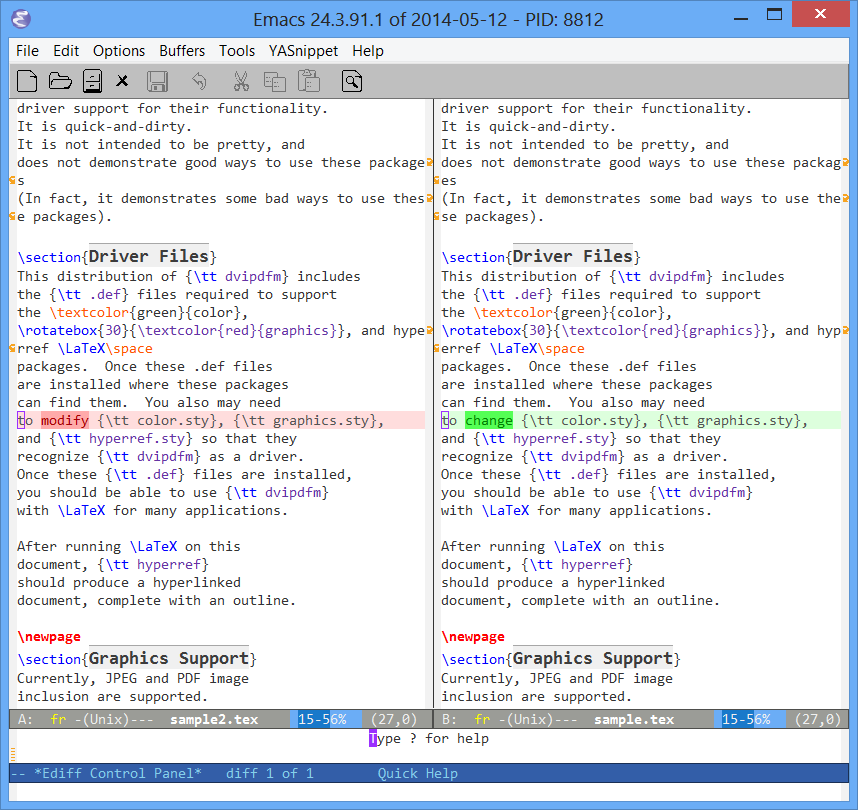
\includegraphics[width=.65\linewidth]{images/ediff.png}
\end{figure}
\end{frame}

\begin{frame}[label={sec:orgfcf70f1}]{Dired}
\begin{figure}[!htbp]
\centering
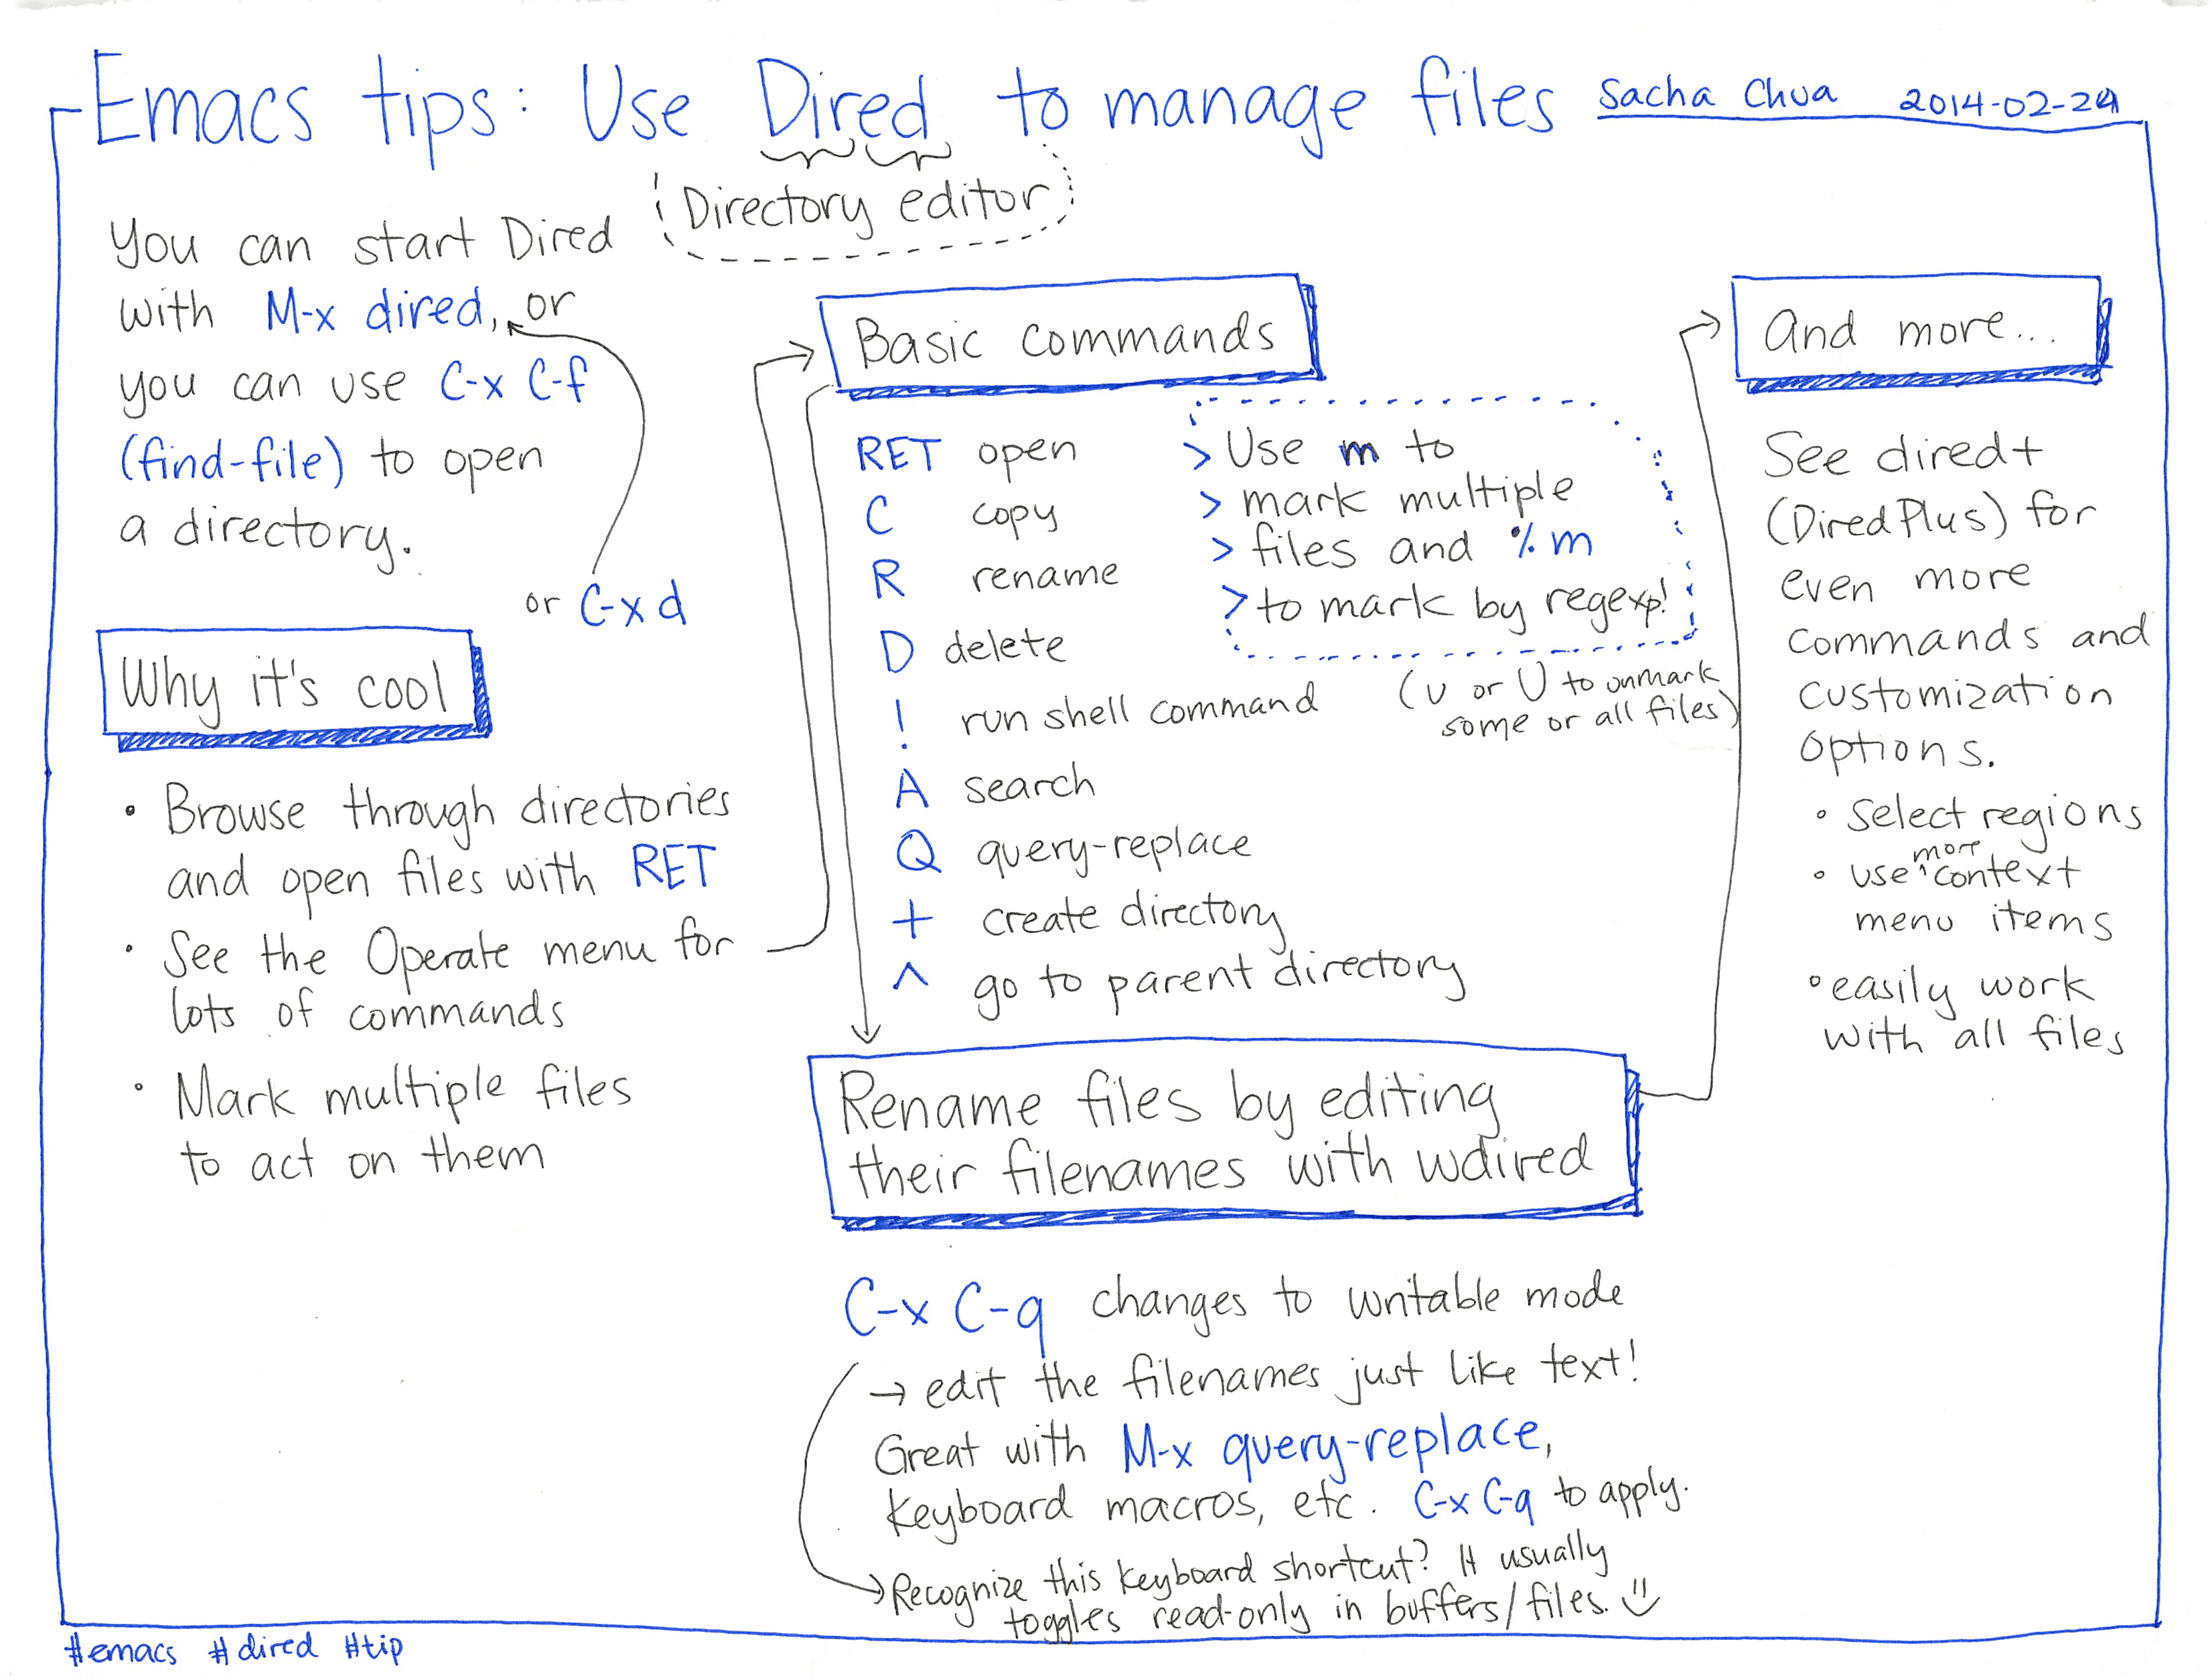
\includegraphics[width=.75\linewidth]{images/2014-02-24-Emacs-tips-use-Dired-to-manage-files-dired-emacs.png}
\end{figure}
\end{frame}

\begin{frame}[fragile,label={sec:orgae1b201}]{Dictionary mode}
 \lstset{language=Lisp,label= ,caption= ,captionpos=b,numbers=none}
\begin{lstlisting}
;; Client for rfc2229 dictionary servers.
(when (require "dictionary-autoloads" nil t)

  (global-set-key
    (kbd "C-c d s") 'dictionary-search)
  (global-set-key
    (kbd "C-c d l") 'dictionary-lookup-definition)
  (global-set-key
    (kbd "C-c d m") 'dictionary-match-words)

  (with-eval-after-load "dictionary"

    (global-dictionary-tooltip-mode 1)

    ;; ;; Server contacted for searching the dictionary.
    ;; (setq dictionary-server "localhost")

  ))
\end{lstlisting}
\end{frame}

\begin{frame}[fragile,label={sec:org8aa9659}]{Highlight line}
 \lstset{language=Lisp,label= ,caption= ,captionpos=b,numbers=none}
\begin{lstlisting}
(require 'hl-line)
(hl-line-mode)
\end{lstlisting}
\end{frame}

\section{Conclusions}
\label{sec:org2cfab9e}

\begin{frame}[label={sec:org7ba421e}]{Continuer à apprendre}
\begin{itemize}
\item Lire la documentation (\href{http://www.gnu.org/software/emacs/}{GNU Emacs}, \href{http://www.emacswiki.org/}{EmacsWiki}, etc.)
\item Étudier les configurations des autres (\href{https://github.com/fniessen/emacs-leuven}{Emacs Leuven}, \href{http://www.dotemacs.de/}{Dot emacs}, etc.)
\item Regarder des tutoriels vidéo (\href{http://www.emacsrocks.com/}{Emacs Rocks}, etc.)
\end{itemize}
\end{frame}

\begin{frame}[label={sec:orgbf7c0db}]{Ne pas se laisser intimider}
\ldots{} par la courbe d'apprentissage

\begin{figure}[!htbp]
\centering
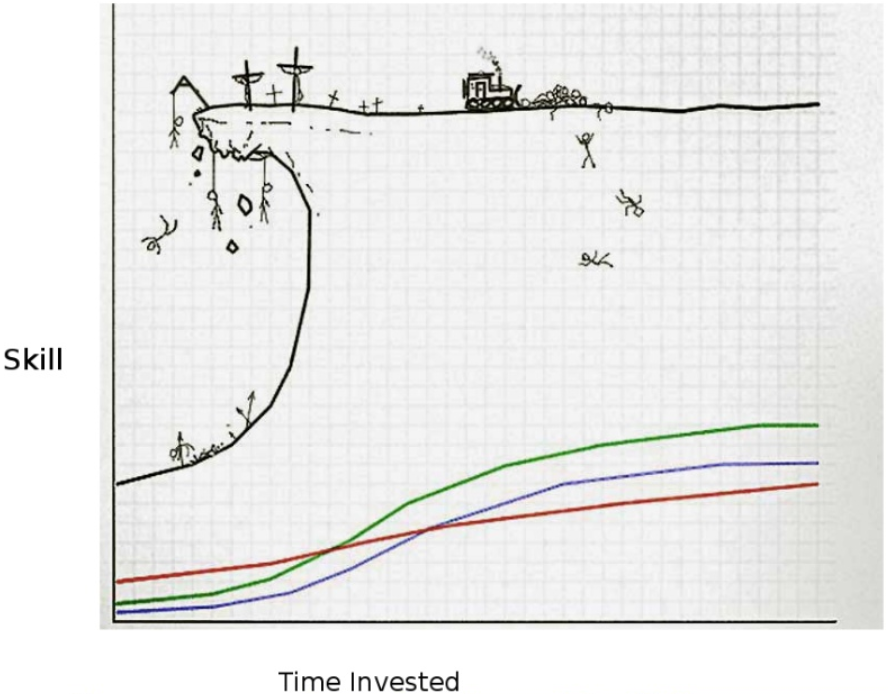
\includegraphics[width=.52\linewidth]{images/courbe-apprentissage.png}
\end{figure}

Apprendre Emacs n'est pas facile (n'est pas compliqué non plus), \\
mais \alert{vous ne le regretterez jamais} !
\end{frame}

\begin{frame}[fragile,label={sec:org506305e}]{Coordonnées}
 Consultant IT @ \href{http://www.pirilampo.be/}{Pirilampo SPRL} \\
Auteur @ \href{http://www.pirilampo.org/}{Pirilampo.org}

\vfill{}

\begin{columns}
\begin{column}{0.48\columnwidth}
\begin{center}
\begin{tabular}{ll}
\href{https://github.com/fniessen}{GitHub} & \texttt{fniessen}\\
\href{http://be.linkedin.com/pub/fabrice-niessen/0/a42/200}{LinkedIn} & \texttt{fabrice-niessen}\\
\href{http://www.slideshare.net/fniessen}{SlideShare} & \texttt{fniessen}\\
\href{https://twitter.com/f\_niessen}{Twitter} & \texttt{f\_niessen}\\
\end{tabular}
\end{center}
\end{column}

\begin{column}{0.48\columnwidth}
\begin{center}
\begin{tabular}{l}
Vous avez des idées~?\\
Contactez-moi~!\\
\end{tabular}
\end{center}
\end{column}
\end{columns}
\end{frame}
\end{document}
